\documentclass[sigconf,nonacm]{acmart}
\makeatletter
\renewcommand\@formatdoi[1]{\ignorespaces}
\makeatother


\AtBeginDocument{\providecommand\BibTeX{{\normalfont B\kern-0.5em{\scshape i\kern-0.25em b}\kern-0.8em\TeX}}}


\acmDOI{}
\acmISBN{}


\usepackage{hyperref}
\usepackage{siunitx}
\usepackage{xspace}
\usepackage{multirow}
\usepackage{enumitem}
\usepackage{placeins}
\usepackage{natbib}
\newcommand{\ours}{\textsc{TinyLLM}\xspace}
\settopmatter{printacmref=false}
\setcopyright{none}
\pagestyle{plain}


\begin{document}


\title{\ours: Learning a Small Student from Multiple Large Language Models}


\author{Yijun Tian}
\authornote{Equally contributed.}
\affiliation{\institution{University of Notre Dame}
  \country{}
}
\email{yijun.tian@nd.edu}

\author{Yikun Han}
\authornotemark[1]
\affiliation{\institution{University of Michigan}
  \country{}
}
\email{yikunhan@umich.edu}

\author{Xiusi Chen}
\authornotemark[1]
\affiliation{\institution{University of California, Los Angeles}
  \country{}
}
\email{xchen@cs.ucla.edu}


\author{Wei Wang}
\affiliation{\institution{University of California, Los Angeles}
  \country{}
}
\email{weiwang@cs.ucla.edu}


\author{Nitesh V. Chawla}
\affiliation{\institution{University of Notre Dame}
  \country{}
}
\email{nchawla@nd.edu}


\begin{abstract}
  Transferring the reasoning capability from stronger large language models (LLMs) to smaller ones has been quite appealing, as smaller LLMs are more flexible to deploy with less expense. Among the existing solutions, knowledge distillation stands out due to its outstanding efficiency and generalization. However, existing methods suffer from several drawbacks, including limited knowledge diversity and the lack of rich contextual information. To solve the problems and facilitate the learning of compact language models, we propose \ours, a novel knowledge distillation paradigm to learn a small student LLM from multiple large teacher LLMs. In particular, we encourage the student LLM to not only generate the correct answers but also understand the rationales behind these answers. Given that different LLMs possess diverse reasoning skills, we guide the student model to assimilate knowledge from various teacher LLMs. We further introduce an in-context example generator and a teacher-forcing Chain-of-Thought strategy to ensure that the rationales are accurate and grounded in contextually appropriate scenarios. Extensive experiments on six datasets across two reasoning tasks demonstrate the superiority of our method. Results show that \ours can outperform large teacher LLMs significantly, despite having a considerably smaller model size.
\end{abstract}


\maketitle


\section{Introduction}
Large language models (LLMs) have recently taken over various domains and applications, including society ~\cite{rao2023makes}, education~\cite{zelikman2023generating}, and scientific understanding~\cite{beltagy2019scibert}. Despite the success of larger emerging models (GPT-4, Claude-2), their smaller counterparts hardly demonstrate such promising capabilities for performing complex reasoning~\cite{wei2022emergentabilities,chen2023gotta}. This has been unveiled as the well-known scaling law of LLMs~\cite{kaplan2020scalinglaws}. As such, it has been desirable to transfer the capabilities of the larger models to the smaller ones so that the smaller ones could be easily deployed while still enjoying the strong capabilities. Previous studies have shown that knowledge distillation is an instrumental tool in mitigating the performance gap between larger models such as LLMs and smaller ones~\cite{wan2023efficient, hsieh-etal-2023-distilling, kd_survey}. Examples of effective distillation methods include DistilBERT~\cite{sanh2019distilbert}, Alpaca~\cite{alpaca} and Vicuna~\cite{zheng2023judging}.


However, existing methods suffer from two major drawbacks: (1) \textbf{Limited Knowledge Diversity}: Current research predominantly employs a single-teacher approach, which confines the learning scope of the student model to the knowledge derived from its own training and architecture designs \cite{ho2022largelanguagemodels,magister2022teachingsmall,li2023symbolicchain,wang2022pinto}. This means that the student model is limited to the perspectives, biases, and potential weaknesses of the teacher. (2) \textbf{Lack of Rich Contextual Information}: While rationales play a vital role in effective reasoning \cite{wei2022chainofthought,kojima2022zero}, current research primarily focuses on leveraging ground truth labels, which indicate the correct answer but do not provide insights into the reasoning and thought process behind that answer.


In response to the above issues, we propose \ours, a paradigm that improves the reasoning ability of small student LLMs by distilling knowledge from multiple large teacher LLMs with rationale guidance. Specifically, \ours mitigates the limited knowledge diversity issue by involving multiple teacher models as \textit{co-advisors}. To fully exploit each teacher model and mitigate the lack of rich contextual information problem, \ours asks the teacher for the rationales to support the answers. By learning from multiple teachers, the student model can inherit a broader range of skills and knowledge, leading to better generalization capabilities. In addition, to ensure the rationales are grounded in contextually appropriate scenarios and reflect the true underlying reasoning procedure, \ours features an in-context example generator and a teacher-forcing Chain-of-Thought strategy, making the teachers understand the task through demonstrations and generate the accurate rationales.


To thoroughly assess our approach, we conduct experiments on six datasets in commonsense and biomedical reasoning tasks. The results show that the usage of our paradigm enhances performance by \textbf{+5.07\%} to \textbf{+12.57\%} compared to full fine-tuning with significantly smaller model size, i.e., \textbf{1.1\%} to \textbf{26.0\%} of teacher sizes. We also perform ablation studies to demonstrate the validity of teacher rationales and undertake hyperparameter analyses for a comprehensive evaluation. To summarize, our main contributions are as follows:


\begin{figure*}[ht]
\begin{center}
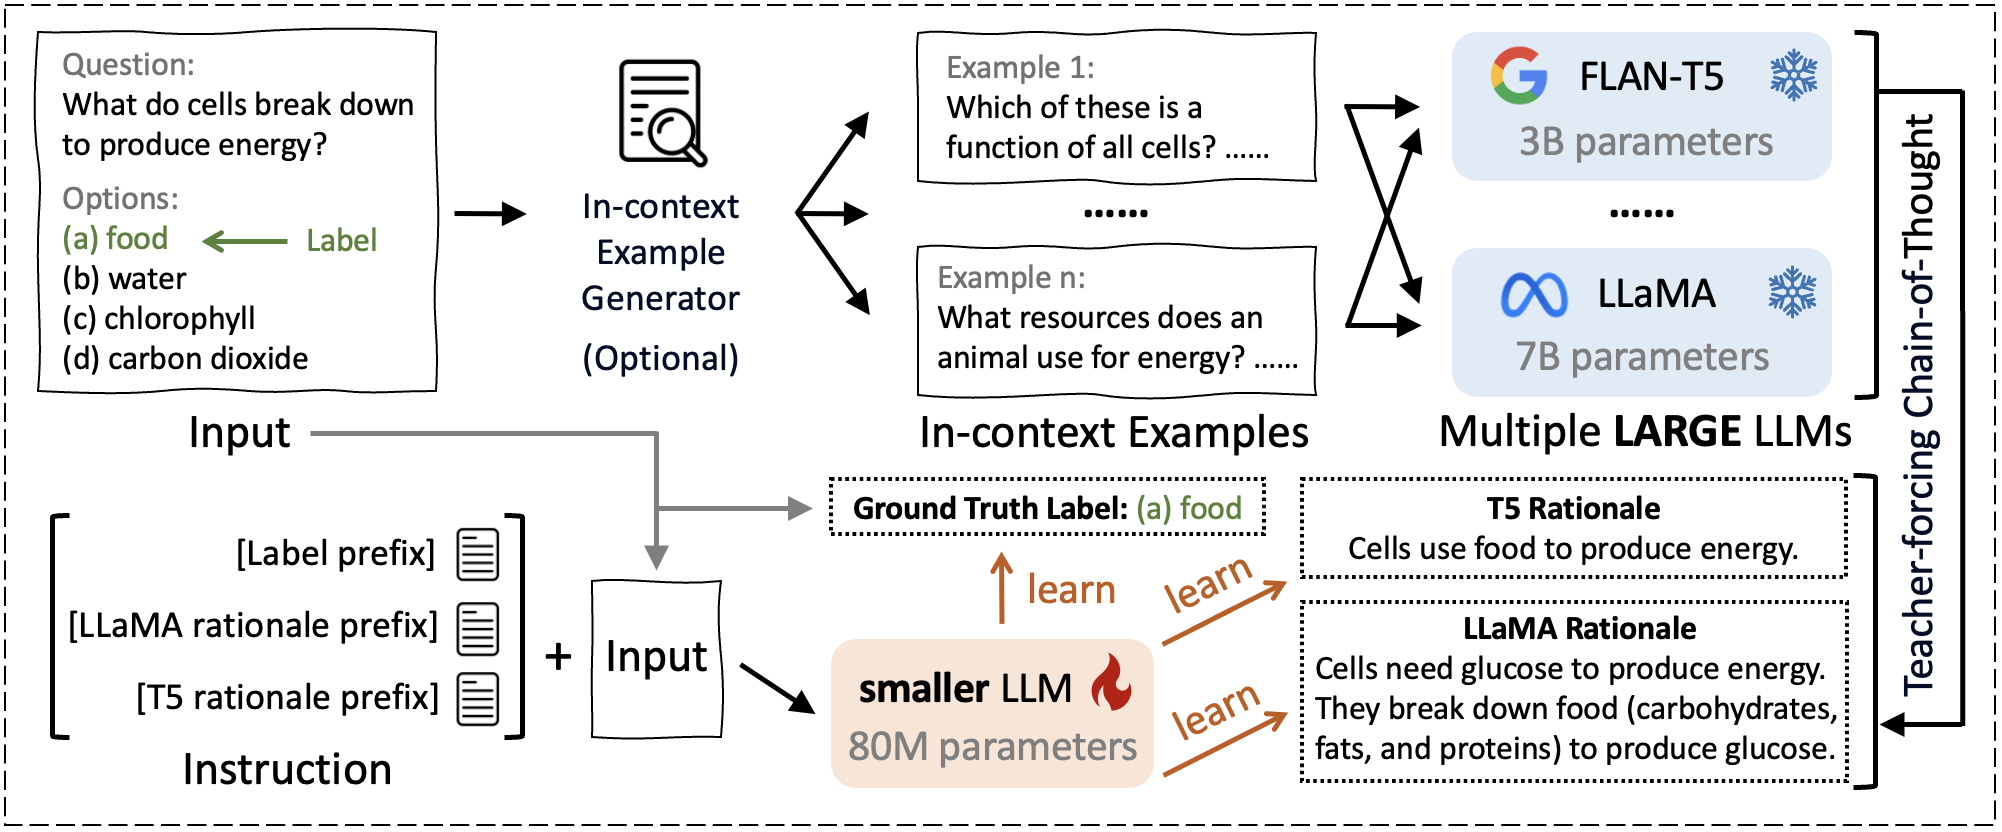
\includegraphics[width=\textwidth]{Figures/pipeline.png}
\end{center}
\vspace{-0.1in}
\caption{
Pipeline of \ours: Given an input question, we first generate in-context examples and obtain rationales from multiple large LLMs via a teacher-forcing Chain-of-Thought Strategy. Later, a small student LLM is trained to integrate rationales from different teachers via multi-task instruction tuning, along with the ground truth label.
}
\label{fig:pipeline}
\vspace{-0.1in}
\end{figure*}


\begin{itemize}[nosep,leftmargin=*]
\item We identify two problems with existing work on learning smaller language models: 1) limited knowledge diversity and 2) lack of rich contextual information.
\item To address the problems, we propose \ours, a novel knowledge distillation paradigm to learn a small student LLM by transferring reasoning capabilities from multiple large teacher LLMs. We encourage the student LLM to understand the rationale behind the generated answer.
\item Extensive experiments validate the superiority of \ours across six datasets and two reasoning tasks. 
\ours can achieve up to \textbf{+12.57\%} of performance improvement with 1.1\% of model size.
\end{itemize}


\section{Method}
The pipeline of \ours is shown in Figure \ref{fig:pipeline}.


\vspace{-0.05in}
\subsection{Preliminary}
\textbf{Multiple Choice Question Answering.} A $k$-way multiple choice question answering (MCQA) is defined as follows: Given a question $Q_i$, a set of candidate answer options $O_i=\{O_{i1},O_{i2},...,O_{ik}\}$, the model is tasked with selecting the correct answer from the set $O_i$, such that the selected answer aligns the ground truth label $A_i$.


\noindent \textbf{Knowledge Distillation.} 
The knowledge distillation process begins with the teacher model, denoted as $T$ parameterized by $\theta_T$, which has been pre-trained on a large corpus. Later, the student model, $S$, with parameter $\theta_S$, is tasked with distilling knowledge directly from $T$, leveraging the strong capabilities of $T$.


\subsection{Obtaining Rationales from Teachers}


\noindent
\textbf{In-context Example Generator.}
To enable the rationales that are generated by teachers to be grounded in contextually appropriate scenarios, we introduce an optional in-context example generator. This tool is designed to produce in-context examples for any given input, providing more detailed information about the input data and task. For simplicity, we select the examples randomly within the same dataset. This aids the teacher LLMs in comprehending the nature and specifics of the task more deeply. By integrating this generator, we facilitate a more informed and nuanced generation of rationales by the teacher models, enhancing the learning experience for the student model. 

\noindent
\textbf{Teacher-forcing Chain-of-Thought.}
In addition, we design a teacher-forcing strategy to ensure the validity of the rationales. Compared to existing methods that simply employ regular chain-of-thought (CoT) mechanisms \cite{wei2022chainofthought,kojima2022zero}, wherein an LLM is prompted with sets of questions and options \(\{Q_i, O_i\}\) to elicit rationales \(R_i\) directly, \ours posits a distinct advantage in integrating the correct answer \(A_i\) into the input. We hypothesize that the inclusion of \(A_i\) alongside \(Q_i\) and \(O_i\) facilitates a more nuanced understanding of the input context and the correct logical rationales leading to the answer, thereby facilitating a more informed and accurate generation process. Specifically, we consider the concatenation of questions, options, and answers \(\{Q_i, O_i, A_i\}\) as the input to LLMs.


\noindent
\textbf{Rationales from Multiple Teachers.}
Given $M$ teachers, \ours pioneers the usage of a multi-teacher architecture in which each teacher \(T^m\) is an LLM. In particular, the rationale \(R_i^m\) produced by a specific teacher model $\theta_{T^m}$ for the \(i\)th question is derived using the question $Q_i$, options $O_i$, correct answer $A_i$, and in-context examples $P_i$. The process is formalized as follows:
\begin{equation}
R_i^m = T^m(Q_i, O_i, A_i, P_i; \theta_{T^m}).
\end{equation}


\begin{table*}[ht]
\caption{Overall experimental results. The best results across different LLM sizes are highlighted in bold. $\Delta_{FF}$ represents the relative performance improvement of \ours to Full Fine-Tuning. Accuracy is used as the evaluation metric.}
\vspace{-0.1in}
\label{Overall}
  \begin{tabular}{ccccccccc}
    \toprule
     &  & \multicolumn{4}{c}{Commonsense Reasoning} & \multicolumn{2}{c}{Biomedical Reasoning} & \\ 
    \cmidrule{3-8}
    \multirow{-2.3}{*}{\textbf{LLM}}  & \multirow{-2.3}{*}{\textbf{Method}} & {\textbf{OBQA}} & {\textbf{ARC}} & {\textbf{PIQA}} & {\textbf{Riddle}} & {\textbf{PQA}} & {\textbf{BioASQ}} & \multirow{-2.3}{*}{\textbf{Total}}\\
    \midrule
    \multirow{2}{*}{3B/7B Teacher} & FLAN-T5 xlarge & 69.20 & 68.24 & 58.43 & 53.73 & 71.50 & 65.85 & 64.49\\
    & LLaMA 2 & 58.60 & 45.90 & 78.80 & 47.65 & 54.50 & 73.75 & 59.87\\
    \midrule
    
    \multirow{5}{*}{\begin{tabular}[c]{@{}c@{}}80M Student\\Size: 2.7\%/1.1\%\end{tabular}} & Inference & 16.60 & 19.31 & 20.78 & 13.33 & 38.00 & 47.97 & 26.00 \\
     &  LoRA & 37.80 & 27.12 & 39.93 & 39.80 & 53.75 & 78.05 & 46.08 \\
     &  {Full Fine-tuning} & 41.60 & 27.47 & 42.33 & 42.75 & 56.25 & 78.86 & 48.21\\
     &  {\ours} & \textbf{47.60} & \textbf{31.93} & \textbf{52.77} & \textbf{49.22} & \textbf{62.00} & \textbf{82.11} & \textbf{54.27}\\
     &  {$\Delta_{FF}$} & $\uparrow 14.42\%$ & $\uparrow 16.24\%$ & $\uparrow 24.66\%$ & $\uparrow 15.13\%$ & $\uparrow 10.22\%$ & $\uparrow 4.12\%$ & $\uparrow 12.57\%$\\
    \midrule
     
    \multirow{5}{*}{\begin{tabular}[c]{@{}c@{}}250M Student\\Size: 8.3\%/3.6\%\end{tabular}} & Inference & 31.00 & 23.00 & 30.47 & 30.78 & 48.00 & 57.72 & 36.83 \\
    &  LoRA & 51.40 & 37.25 & 47.66 & 53.14 & 62.00 & 82.93 & 55.73\\
    &  {Full Fine-tuning} & 56.60 & 38.88 & 47.55 & 52.55 & 64.75 & 89.43 & 58.29\\
    &  {\ours} & \textbf{64.20} & \textbf{47.98} & \textbf{60.17} & \textbf{60.78} & \textbf{66.25} & \textbf{90.24} & \textbf{64.94}\\
    &  {$\Delta_{FF}$} & $\uparrow 13.43\%$ & $\uparrow 23.41\%$ & $\uparrow 26.54\%$ & $\uparrow 15.66\%$ & $\uparrow 2.32\%$ & $\uparrow 0.91\%$ & $\uparrow 11.40\%$\\
    \midrule
    
    \multirow{5}{*}{\begin{tabular}[c]{@{}c@{}}780M Student\\Size: 26.0\%/11.1\%\end{tabular}} & Inference & 50.40 & 51.07  & 51.90 & 39.80 & 64.25 & 63.41 & 53.47\\
    &  LoRA & 64.00 & 57.77 & 57.02 & 68.63 & 70.25 & 86.18 & 67.31\\
    &  {Full Fine-tuning} & 71.20 & 62.92 & 58.43 & 68.82 & 70.25 & 90.24 & 70.31\\
    & {\ours} & \textbf{74.40} & \textbf{64.29} & \textbf{67.90} & \textbf{70.98} & \textbf{73.00} & \textbf{92.68} & \textbf{73.88}\\
    &  {$\Delta_{FF}$} & $\uparrow 4.49\%$ & $\uparrow 2.18\%$ & $\uparrow 16.21\%$ & $\uparrow 3.14\%$ & $\uparrow 3.91\%$ & $\uparrow 2.70\%$ & $\uparrow 5.07\%$\\
    
    \bottomrule
  \end{tabular}
\end{table*}


\subsection{Learning a Small Student}
A straightforward strategy to incorporate rationales as supervision is to append each rationale \(R_i^m\) generated by the teacher models as supplementary input to the student model, along with the question \(Q_i\) and options \(O_i\). However, this method faces challenges due to limitations in computational resources at the inference stage, especially because rationales must be pre-generated for every data sample in both training and test sets~\cite{wang2022pinto}. To overcome this issue, we employ rationales as a form of supervisory signal during the training process to develop a model that is adept at generating its own explanations. Subsequently, this trained model can be utilized on the test set, eliminating the need for pre-generated rationales to facilitate accurate reasoning. Specifically, \ours integrates rationales from multiple teacher models into a unified multi-task instruction tuning framework. This necessitates the assignment of a unique prefix \(p\) for distinguishing between learning tasks from different teachers. The student model is trained not only to predict labels but also to generate rationales akin to those produced by the teachers. Accordingly, the overall loss function $\mathcal{L}$ is as follows:
\begin{equation}
\mathcal{L} = \mathcal{L}_A + \sum_{m=1}^{M}\alpha^m\mathcal{L}_{T^m}, 
\label{eq:total_loss}
\end{equation}
where \(\mathcal{L}_A\) denotes the objective of learning from ground truth answers, $\mathcal{L}_{T^m}$ indicates the objective of learning from $m$-th teacher, $\alpha^m$ is the importance weight for $T^m$, and $M$ is the number of teacher LLMs. Formally, $\mathcal{L}_A$ and $\mathcal{L}_{T^m}$ are defined as follows:
\begin{equation}
\mathcal{L}_A = \frac{1}{N} \sum_{i=1}^{N} \ell(S(Q_i, O_i, p_A; \theta_S), A_i),
\end{equation}
\begin{equation}
    \mathcal{L}_{T^m} = \frac{1}{N} \sum_{i=1}^{N} \ell(S(Q_i, O_i, p_m; \theta_S), R_i^m),
\end{equation}
where $N$ is the number of data samples, $\ell$ indicates the cross-entropy loss between the predicted and target tokens. Here $\mathcal{L}_A$ encourages the student $S$ to generate ground truth answer $A_i$ by minimizing the difference between it and the student output given the question $Q_i$, options $O_i$, and instruction prefix $p_A$ for generating answers. On the other hand, $\mathcal{L}_T^m$ facilitates the student $S$ to mimic the reasoning capability of teacher $T^m$ by learning from its rationale $R_i^m$, with the guidance of instruction prefix $p_m$ for $T^m$.


\section{Experiments}


\subsection{Experimental Setup}

\textbf{Datasets.} 
We follow the setup in GNP \cite{gnp} for the usage of commonsense reasoning and biomedical reasoning datasets, including OpenBookQA (OBQA)~\cite{OpenBookQA2018}, The AI2 Reasoning Challenge (ARC)~\cite{Clark2018ThinkYH}, Physical Interaction Question Answering (PIQA)~\cite{Bisk2020PIQA}, RiddleSense (Riddle)~\cite{lin-etal-2021-riddlesense}, PubMedQA (PQA)~\cite{jin2019pubmedqa}, and BioASQ~\cite{Tsatsaronis2015BIOASQ}.


\noindent \textbf{Baselines.} 
We benchmark \ours against the teacher's performance and various training approaches, including an Inference configuration without training, an efficient training method LoRA \cite{hu2022lora} that updates a subset of parameters, and the full fine-tuning that updates all the parameters in the student.


\noindent \textbf{Implementation Details.} For \ours, we set the learning rate to \(5 \times 10^{-5}\), batch size to 16, maximum input length to 1024, and epoch to 1. Trade-off weights \(\alpha_{T_n}\) are explored within \{0.01, 0.1, 0.5, 1, 2, 3\}. For the choice of LLMs, we use FLAN-T5 ~\cite{chung2022scaling} small (80M), base (250M), and large (780M) as the student, and FLAN-T5 xlarge (3B) and LLaMA 2-chat ~\cite{touvron2023llama2} (7B) as teachers. Experiments are conducted on four NVIDIA Tesla H100 GPUs.


\subsection{Performance Comparison}
\textbf{Comparison to Students Learning Methods.}
The results of six datasets and two reasoning tasks are shown in Table ~\ref{Overall}. From the table, we observe that the employment of a full-finetuning method, despite its theoretically enhanced capacity for parameter adjustment, does not consistently yield superior results to LoRA. Conversely, \ours demonstrates substantial performance enhancements across all datasets and LLM sizes. In total, \ours achieves an average enhancement of \textbf{+12.57\%}, \textbf{+11.40\%} and \textbf{+5.07\%} for students with 80M, 250M, and 780M parameters, respectively. This validates the effectiveness of \ours and underscores the importance and benefits of learning from teachers.


\noindent \textbf{Comparison to Teachers.} 
\ours also shows superior performance compared to the teacher models. For example, a 780M student can achieve an average performance of 73.88 across different datasets, which is \textbf{+14.56\%} better than the 3B teacher and \textbf{+23.40\%} better than the 7B teacher. Moreover, an even smaller student model with 250M parameters can outperform the teachers (\textbf{+0.70\%} to 3B, \textbf{+16.82\%} to 7B) while using only \textbf{8.3\%} and \textbf{3.6\%} of the teacher parameters.


\vspace{-0.05in}
\subsection{Ablation Study}
For a comprehensive evaluation, we conduct ablation studies to validate the contribution of the in-context example generator and rationales from multiple teachers. To facilitate this, we create three ablation variants of \ours. 
\begin{itemize}[leftmargin=*]
    \item \textbf{w/o in-context} rules out the in-context examples during rationale generation.
    \item \textbf{w/o LLaMa} and \textbf{w/o T5} exclude the rationale supervision from the corresponding teacher model during distillation.
\end{itemize}
Table ~\ref{tab:results} depicts the comparison between the full \ours model and its ablations on the six datasets. According to the table, the decreasing performances of removing the in-context examples and teacher rationales demonstrate their effectiveness in enhancing the model. By combining all the designs, the proposed \ours achieves the best performance. These findings indicate that learning high-quality rationale signals from multiple teachers is beneficial in distilling a small LLM with better reasoning ability.


\begin{table}[t]
  \caption{Impact of in-context examples and contributions of various teachers.}
  \vspace{-0.1in}
  \label{tab:results}
  \resizebox{\linewidth}{!}{
  \begin{tabular}{ccccccc}
    \toprule
    &  \multicolumn{4}{c}{Commonsense} & \multicolumn{2}{c}{Biomedical} \\ 
    \cmidrule{2-7}
    \multirow{-2.3}{*}{\textbf{Variant}} & {\textbf{OBQA}} & {\textbf{ARC}} & {\textbf{PIQA}} & {\textbf{Riddle}} & {\textbf{PQA}} & {\textbf{BioASQ}} \\
    \midrule
    {w/o in-context}  & 73.20 & 63.09 & 66.27 & 69.22 & 70.75 & 86.99 \\
    
    {w/o LLaMA}  & 73.00 & 62.32 & 66.70 & 68.82 & 69.25 & 87.81 \\

    {w/o T5}  & 73.80 & 61.80 & 66.49 & 68.63 & 69.50 & 88.62 \\

    {\ours} & \textbf{74.40} & \textbf{64.29} & \textbf{67.90} & \textbf{70.98} & \textbf{73.00} & \textbf{92.68} \\
    \bottomrule
  \end{tabular}
  }
  \vspace{-0.1in}
\end{table}


\vspace{-0.05in}
\subsection{Parameter Sensitivity}

The exploration of trade-off weights reveals the model's adaptability across different choices of parameter values. We conduct sensitivity experiments on datasets ARC for commonsense reasoning and PQA for biomedical reasoning in ~\ref{fig:sensitivity}. According to the figure, we observe that the optimal parameters for various datasets and tasks differ. The reason for this phenomenon is that biomedical reasoning questions are often lengthy and complex, weakening the impact of rationales from teachers and making a small value of $\alpha$ sufficient. In contrast, commonsense reasoning questions are typically concise and straightforward, making the rationales from teacher models valuable and leading to a large value of $\alpha$.


\begin{figure}[t]
  \centering
  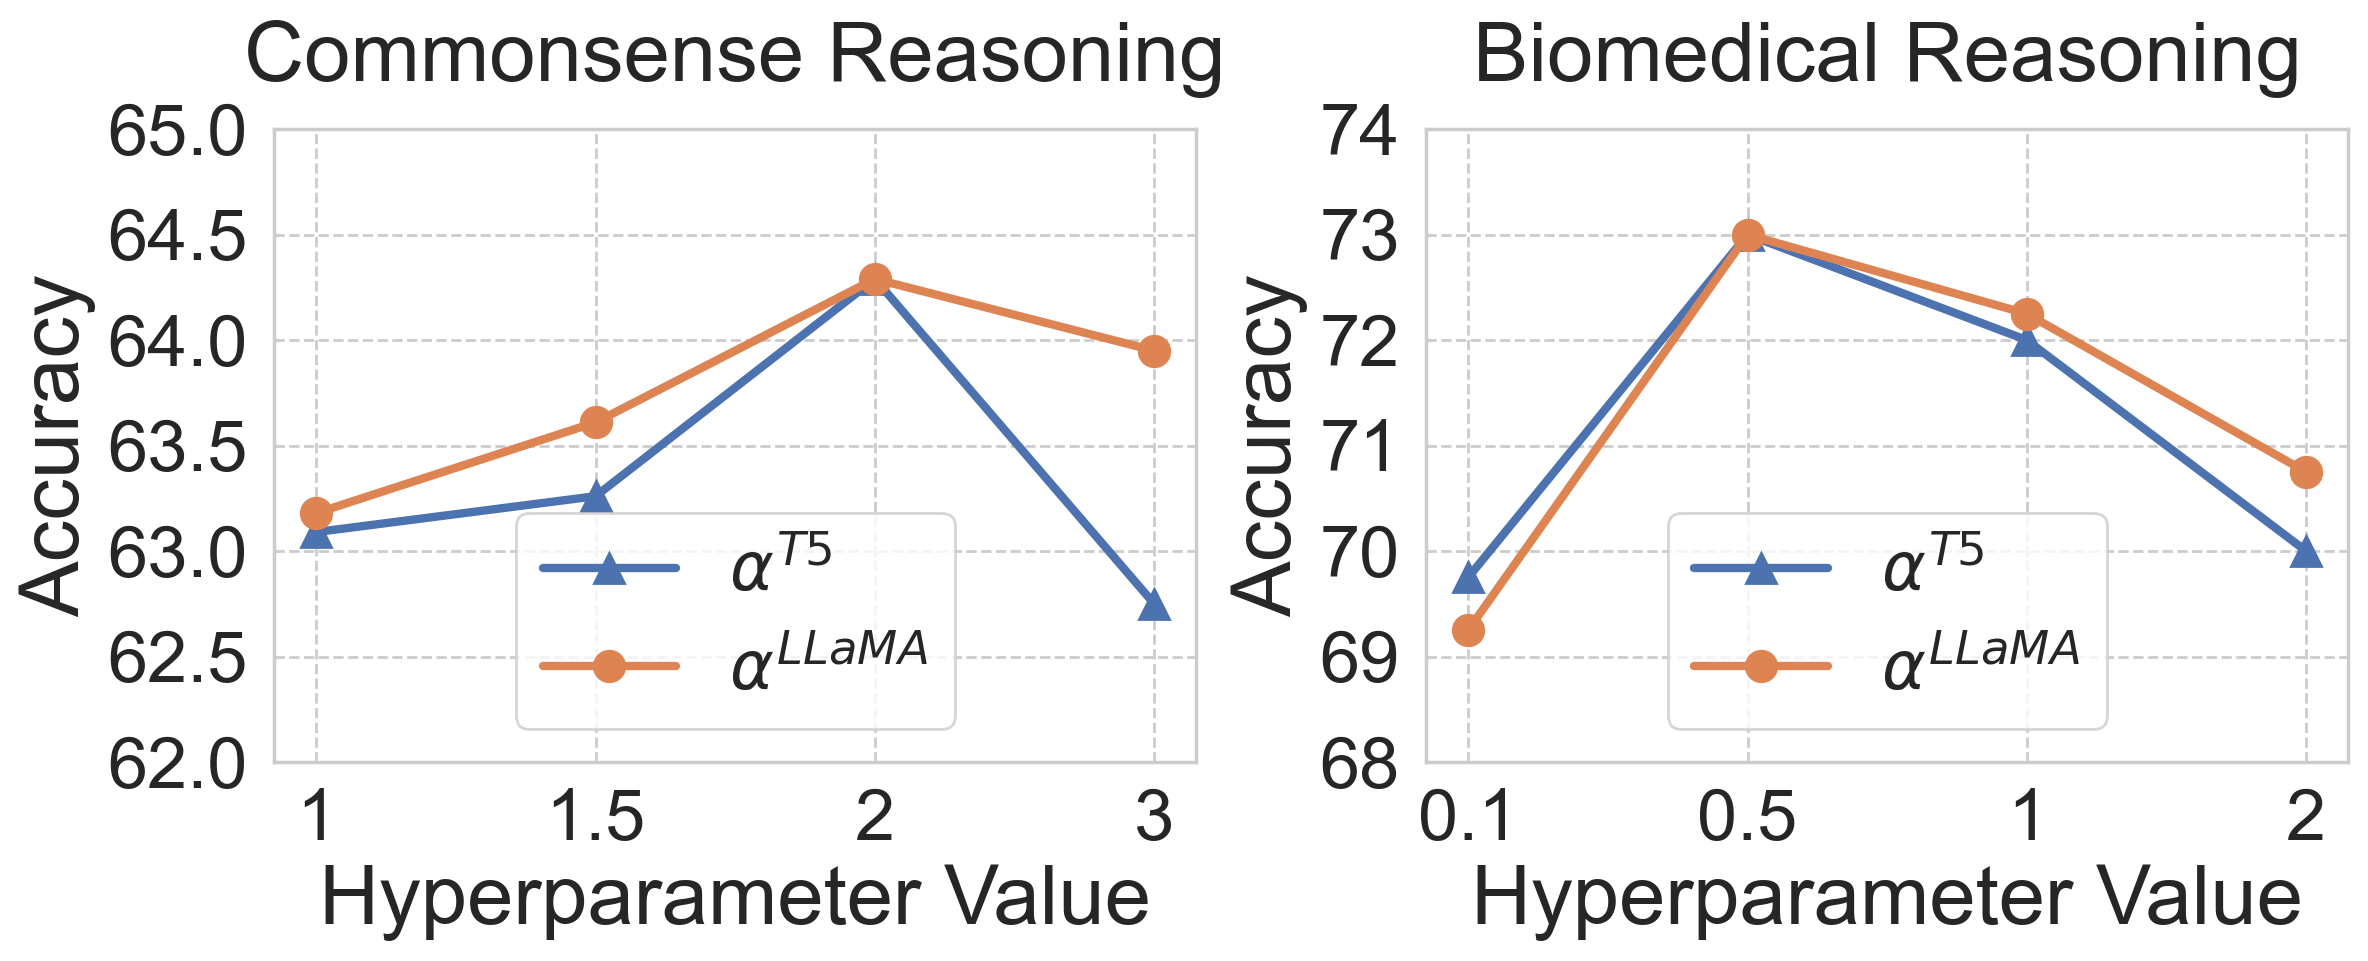
\includegraphics[width=\columnwidth]{Figures/param_sen.png}
  \vspace{-0.25in}
  \caption{Performance w.r.t. different values of weight $\alpha$.}
  \vspace{-0.15in}
  \label{fig:sensitivity}
\end{figure}


\vspace{-0.05in}
\section{Conclusion}
In this paper, we propose \ours, a novel knowledge distillation paradigm to learn a small student LLM from multiple large teacher LLMs. \ours involves several innovative designs, such as inheriting a broader range of knowledge across different teachers and learning contextually appropriate and accurate rationales using an in-context example generator along with a teacher-forcing Chain-of-Thought strategy. Extensive experiments across six datasets and two reasoning tasks validate the superiority of \ours.



\bibliographystyle{acm}
\bibliography{reference}

\end{document}
